\section{Results}

\subsection{Creating a representative dataset of questions}
\label{dataset_results}

We manually create a set of 4760 questions using the method explained in \cref{creating_dataset}.

In order to be able to reuse objects for different questions, we separated the questions and objects in 9 different categories.

\begin{enumerate}
	\item \textbf{Person} Historical people living from early antiquity to the present day from all around the globe. The questions have short, unambiguous answers, such as date of birth or most famous invention.
	\item \textbf{City} Cities from all over the globe. Questions may include population, founding date, notable landmarks, or geographical features.
	\item \textbf{Principle} Scientific principles, discovered from the 16th century forward. Questions about their discovery, use, and others.
	\item \textbf{Element} Elements from the periodic table. Questions may cover discovery, atomic number, chemical properties, or common uses.
	\item \textbf{Book} Literary works from various genres, time periods, and cultures. Questions may involve authors, publication dates, plot summaries, or literary significance.
	\item \textbf{Painting} Famous artworks from different art movements and periods. Questions may cover artists, creation dates, styles, or current locations.
	\item \textbf{Historical Event} Significant occurrences that shaped world history, from ancient times to the modern era. Questions may involve dates, key figures, causes, or consequences.
	\item \textbf{Building} Notable structures from around the world, including ancient monuments, modern skyscrapers, and architectural wonders. Questions may cover location, architect, construction date, or architectural style.
	\item \textbf{Composition} Musical works from various genres and time periods. Questions may involve composers, premiere dates, musical style, or cultural significance.
\end{enumerate}

Each one of these categories has a number of questions that are assigned one of the objects, enhancing the done by \citeauthor{factual_recall}.

The full list of base questions and objects for all categories can be found in \cref{appendixA}.
The total amount of these and composition of the 4760 questions can be found in \cref{category_amounts}.

\begin{table}[ht]
	\centering
	\scriptsize
	\begin{tabular}{>{\bfseries}l r r r}
		\toprule
			\bfseries Category & \bfseries Base Questions & \bfseries Objects & \bfseries Total Questions \\
		\midrule
			Person           &  17 &  57 &  969 \\
			City             &  17 &  70 & 1190 \\
			Principle        &   5 &  37 &  185 \\
			Element          &  15 &  43 &  645 \\
			Book             &  11 &  49 &  539 \\
			Painting         &  12 &  44 &  528 \\
			Historical Event &   4 &  64 &  256 \\
			Building         &   9 &  22 &  198 \\
			Composition      &  10 &  25 &  250 \\
		\midrule
			Total            & 100 & 411 & 4760 \\
		\bottomrule
	\end{tabular}
	\caption{The amount of base questions, objects, and the total amount of questions in each category on the final dataset.}
	\label{category_amounts}
\end{table}

\newpage{}

\subsection{When does a model choose the provided context knowledge over its inherent knowledge?}

The results of running the queries created in \cref{creating_dataset} with added counterparametric context on each of the four models the four models can be found in \cref{total_table,total_results}.

\begin{table}[htbp]
	\centering
	\footnotesize
	\begin{tabular}{l r r r}
		\toprule
			\bfseries Model & \Parametric{} & \Contextual{} & \Other{} \\
		\midrule
			\ttfamily llama-3.1-8B & 745 & 3662 & 353 \\
			\ttfamily llama-3.1-70B & 1070 & 3303 & 387 \\
		\midrule
			\ttfamily flan-t5-xl  & 248 & 4284 & 228 \\
			\ttfamily flan-t5-xxl & 242 & 4304 & 214 \\
		\bottomrule
	\end{tabular}
	\caption{Results when running all entries on a decoder-only model.}
	\label{total_table}.
\end{table}

\begin{figure}[H]
	\centering
	\subfigure[Decoder-only models]{
		\raggedright
		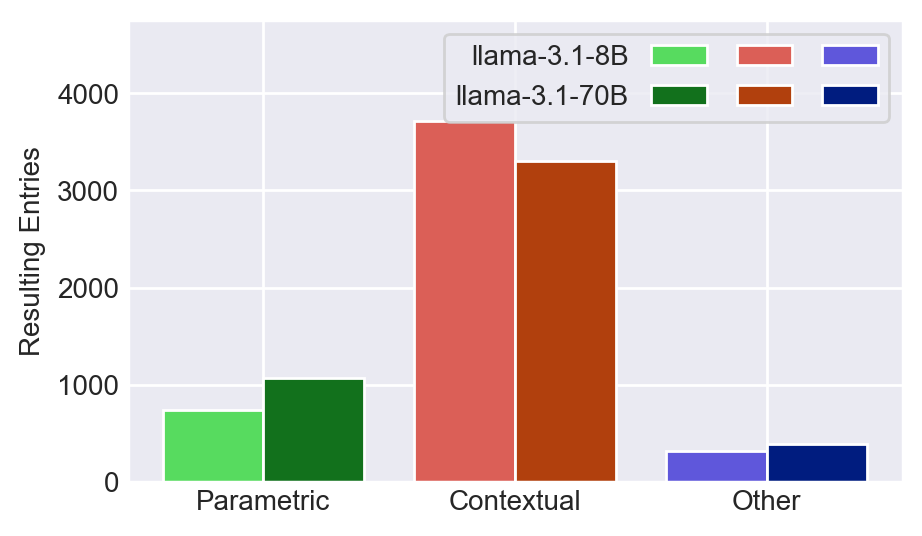
\includegraphics[width=.48\textwidth]{llama_amount.png}
	}%
	\subfigure[Seq2Seq models]{
		\raggedleft
		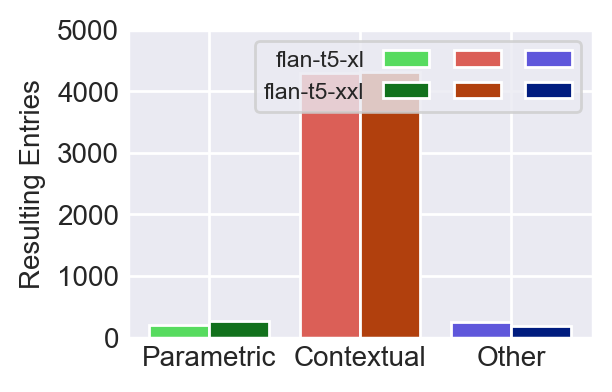
\includegraphics[width=.48\textwidth]{flan_amount.png}
	}
	\caption{Results by type depending on which model; these are the same results as \cref{total_table}.}
	\label{total_results}
\end{figure}

As hypothesised in \cref{intro_models_numbers}, there are vast differences on how the models of different types and sizes act when presented with a context that contradicts their knowledge.
This is investigated further in \cref{discussion}.

A similar pattern emerges in most (but not all) of the categories, which can be seen in \cref{llama_cats_table,llama_cats_result,flan_cats_table,flan_cats_result}.

\begin{table}[htbp]
	\centering
	\footnotesize
	\begin{tabular}{>{\bfseries}l | r r r | r r r}
		\toprule
			& \multicolumn{3}{c|}{\ttfamily \bfseries llama-3.1-8B} & \multicolumn{3}{c}{\ttfamily \bfseries llama-3.1-70B} \\
			& \Parametric{} & \Contextual{} & \Other{} & \Parametric{} & \Contextual{} & \Other{} \\
		\midrule
			Person           &  40 &  833 & 96 & 209 & 614 & 146 \\
			City             & 117 & 1007 & 66 & 166 & 966 &  58 \\
			Principle        &  44 &  118 & 23 &  44 & 117 &  24 \\
			Element          & 218 &  385 & 42 & 275 & 347 &  23 \\
			Book             & 135 &  344 & 60 & 154 & 318 &  67 \\
			Painting         &  47 &  458 & 23 &  49 & 445 &  34 \\
			Historical Event &  81 &  154 & 21 & 117 & 118 &  21 \\
			Building         &  27 &  163 &  8 &  31 & 159 &   8 \\
			Composition      &  36 &  200 & 14 &  25 & 219 &   6 \\
		\bottomrule
	\end{tabular}
	\caption{Results for running each one of the 10 categories separately on the Decoder-only models.}
	\label{llama_cats_table}
\end{table}

\begin{figure}[p]
	\centering
	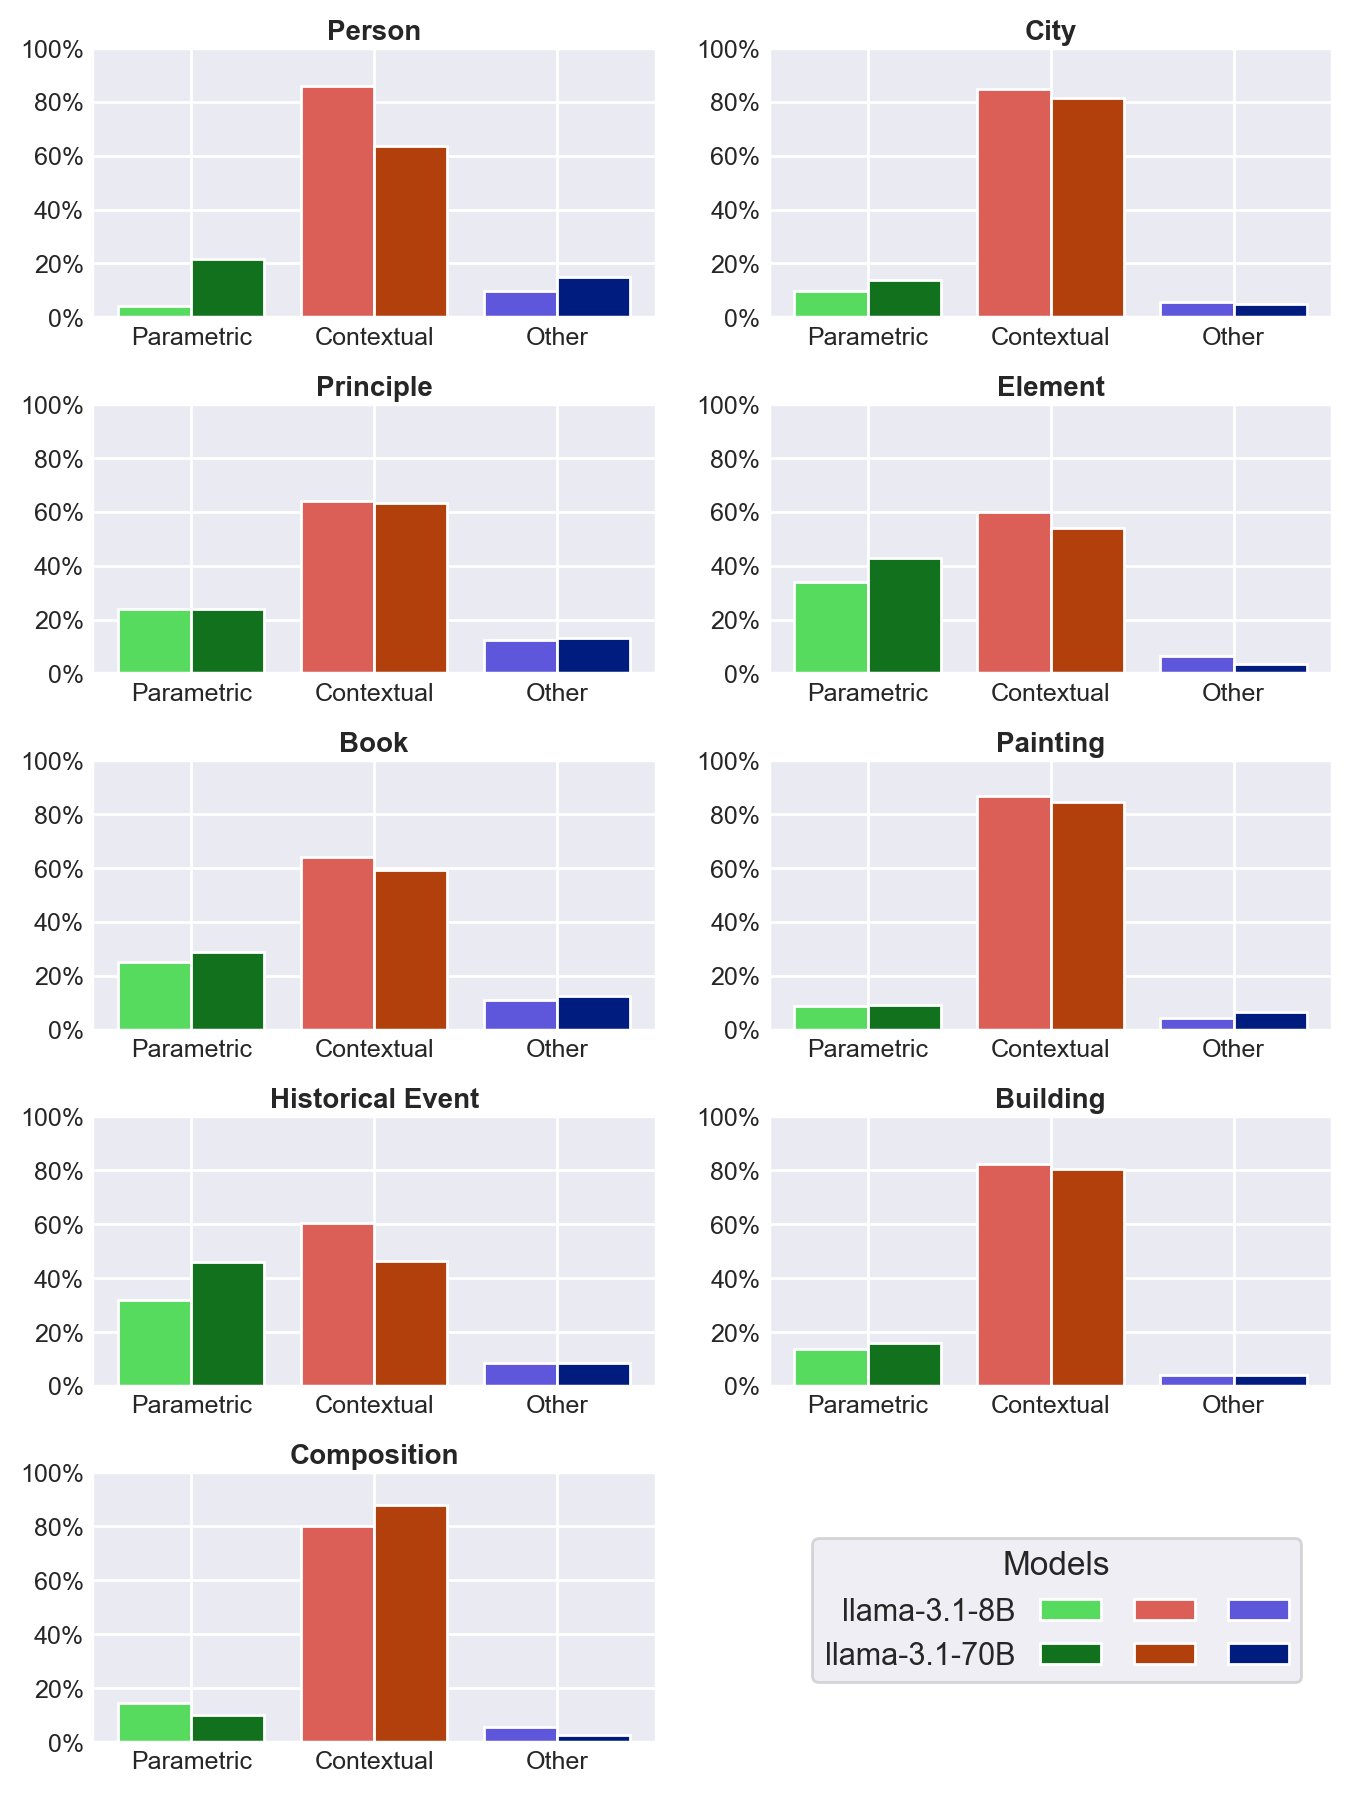
\includegraphics[width=\textwidth]{llama_allcats.png}
	\caption{Results of running decoder-only models on the queried data, grouped by category. This plots the information shown in \cref{llama_cats_table}.}
	\label{llama_cats_result}
\end{figure}

\begin{table}[ht]
	\centering
	\footnotesize
	\begin{tabular}{>{\bfseries}l | r r r | r r r}
		\toprule
			& \multicolumn{3}{|c}{\ttfamily flan-t5-xl} & \multicolumn{3}{|c}{\ttfamily flan-t5-xxl} \\
			& \Parametric{} & \Contextual{} & \Other{} & \Parametric{} & \Contextual{} & \Other{} \\
		\midrule
			Person           &  32 &  900 & 37 &  23 &  890 & 56 \\
			City             & 120 & 1030 & 40 &  78 & 1093 & 19 \\
			Principle        &  13 &  164 &  8 &   9 &  168 &  8 \\
			Element          &   6 &  637 &  2 & 102 &  515 & 28 \\
			Book             &  26 &  488 & 25 &  18 &  457 & 64 \\
			Painting         &  26 &  446 & 56 &   4 &  498 & 26 \\
			Historical Event &  11 &  217 & 28 &   1 &  254 &  1 \\
			Building         &  14 &  174 & 10 &   0 &  189 &  9 \\
			Composition      &   0 &  228 & 22 &   7 &  240 &  3 \\
		\bottomrule
	\end{tabular}
	\caption{Results for running each one of the 10 categories separately on the Seq2Seq models.}
	\label{flan_cats_table}
\end{table}

\begin{figure}[p]
	\centering
	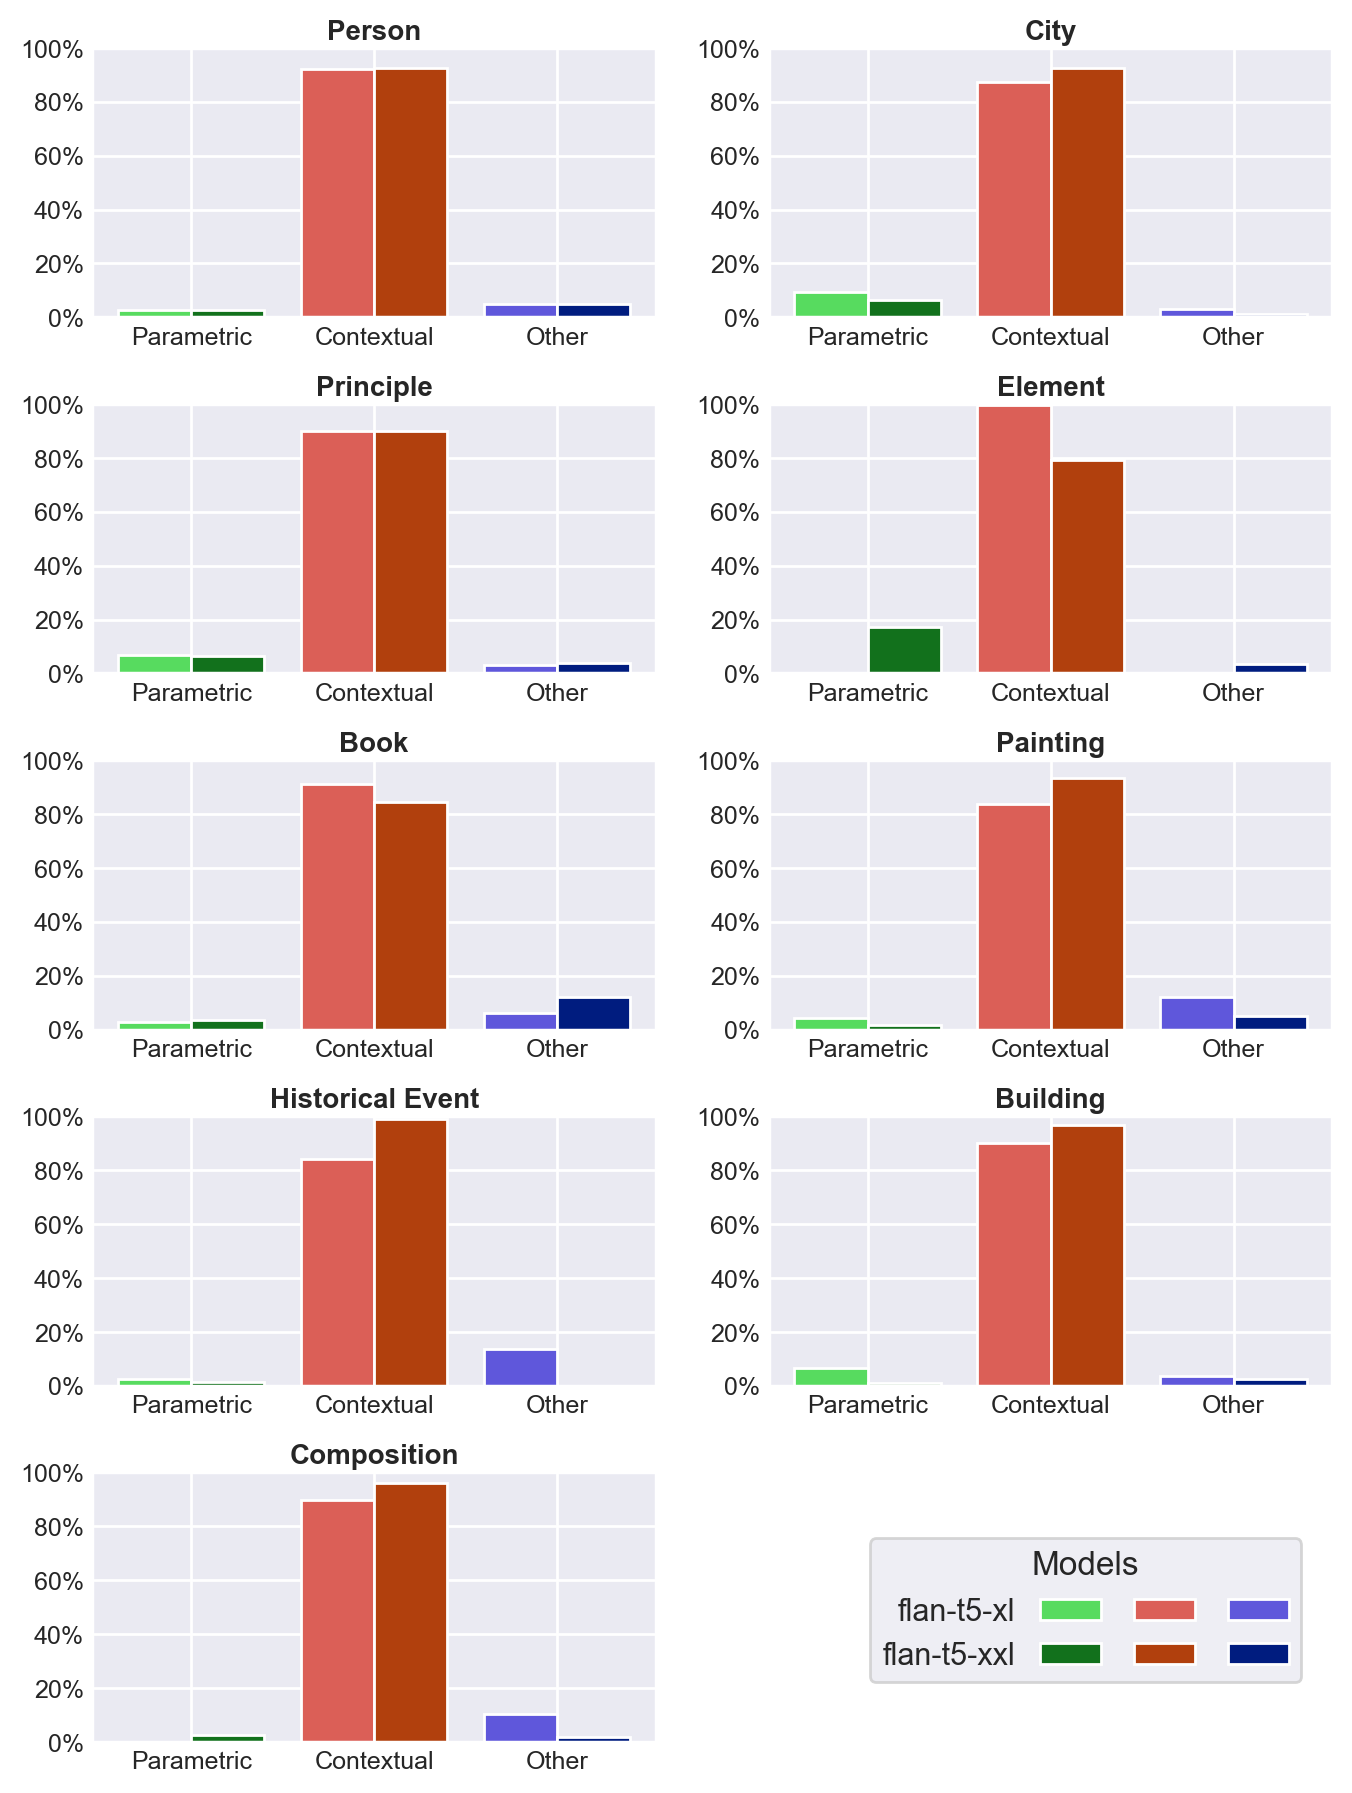
\includegraphics[width=\textwidth]{flan_allcats.png}
	\caption{Results of running Seq2Seq models on the queried data, grouped by category. This plots the information shown in \cref{flan_cats_table}.}
	\label{flan_cats_result}
\end{figure}

\newpage{}

\subsection{Can we use the perplexity score of an answer to predict whether it came from inherent or contextual knowledge?}
\label{results_perplexity_score}

We calculate the resulting perplexity of each query as explained in \cref{method_perplexity}.
These are accumulated in three distributions, depending on answer type, which are summarised in \cref{perplexity_llama_table,perplexity_flan_table,perplexity_results}.

\begin{table}[ht]
	\centering
	\footnotesize
	\begin{tabular}{>{\bfseries}l | r r | r r}
		\toprule
			& \multicolumn{2}{|c}{\ttfamily llama-3.1-8B} & \multicolumn{2}{|c}{\ttfamily llama-3.1-70B} \\
			& \Parametric{} & \Contextual{} & \Parametric{} & \Contextual{} \\
		\midrule
			count &  313 & 4447 &  383 & 4377  \\
			mean  & 1.67 & 1.20 & 1.56 & 1.22  \\
			std   & 0.79 & 0.32 & 0.46 & 0.31  \\
			25\%  & 1.28 & 1.05 & 1.28 & 1.06  \\
			50\%  & 1.43 & 1.10 & 1.43 & 1.12  \\
			75\%  & 1.78 & 1.23 & 1.68 & 1.25  \\
		\bottomrule
	\end{tabular}
	\caption{Distribution of perplexity values for Decoder-only models}
	\label{perplexity_llama_table}
\end{table}

\begin{table}[ht]
	\centering
	\footnotesize
	\begin{tabular}{>{\bfseries}l | r r | r r}
		\toprule
			& \multicolumn{2}{|c}{\ttfamily flan-T5-XL} & \multicolumn{2}{|c}{\ttfamily flan-T5-XXL} \\
			& \Parametric{} & \Contextual{} & \Parametric{} & \Contextual{} \\
		\midrule
			count &  651 & 4109 &   507 & 4253 \\
			mean  & 6.38 & 1.56 & 11.75 & 1.27 \\
			std   & 9.07 & 0.56 & 18.47 & 0.75 \\
			25\%  & 3.21 & 1.19 &  2.41 & 1.02 \\
			50\%  & 4.71 & 1.39 &  3.89 & 1.09 \\
			75\%  & 7.14 & 1.71 &  7.70 & 1.24 \\
		\bottomrule
	\end{tabular}
	\caption{Distribution of perplexity values for Seq2Seq models}
	\label{perplexity_flan_table}
\end{table}

\begin{figure}[H]
	\centering
	\subfigure[Decoder-only models]{
		\raggedright
		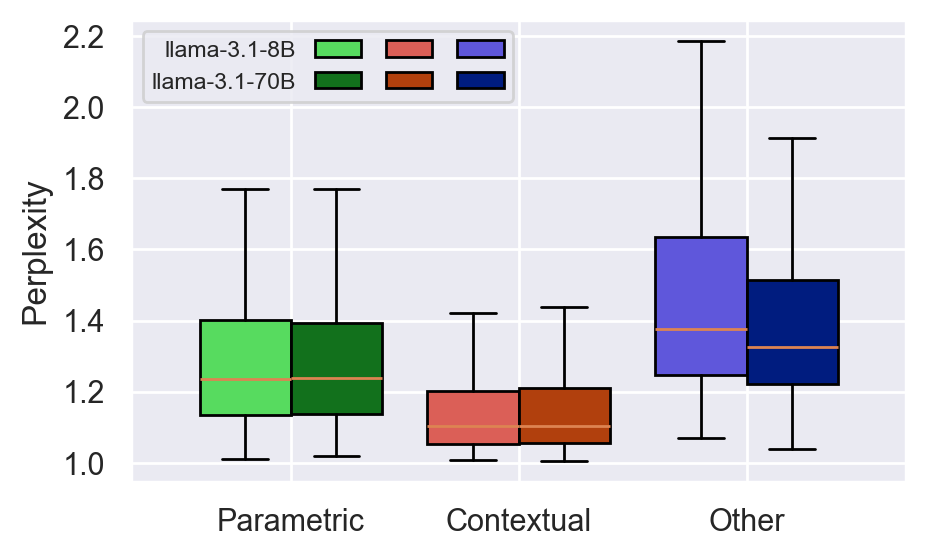
\includegraphics[width=.48\textwidth]{llama_boxplot.png}
	}%
	\subfigure[Seq2Seq models]{
		\raggedleft
		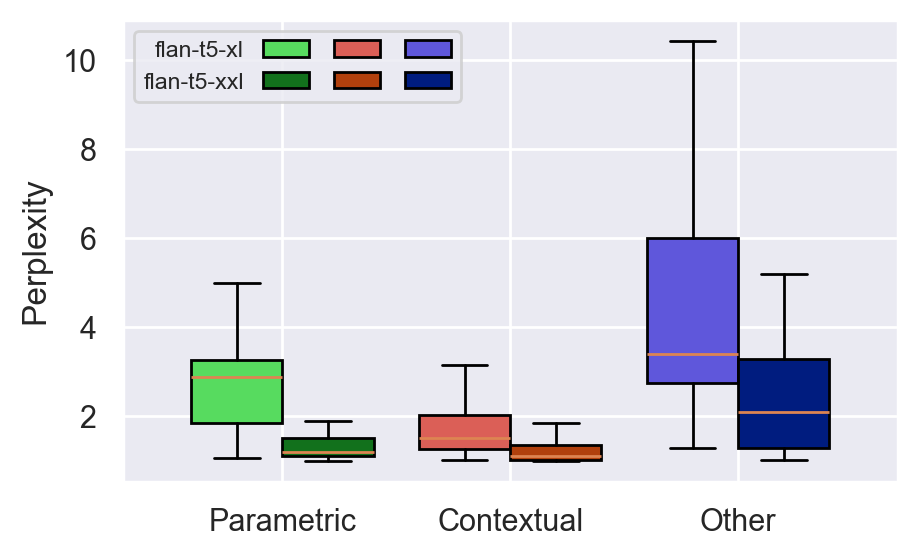
\includegraphics[width=.48\textwidth]{flan_boxplot.png}
	}
	\caption{Perplexity distribution according to model type and size. These represent the same distributions as \cref{perplexity_llama_table,perplexity_flan_table}.}
	\label{perplexity_results}
\end{figure}

\begin{figure}[p]
	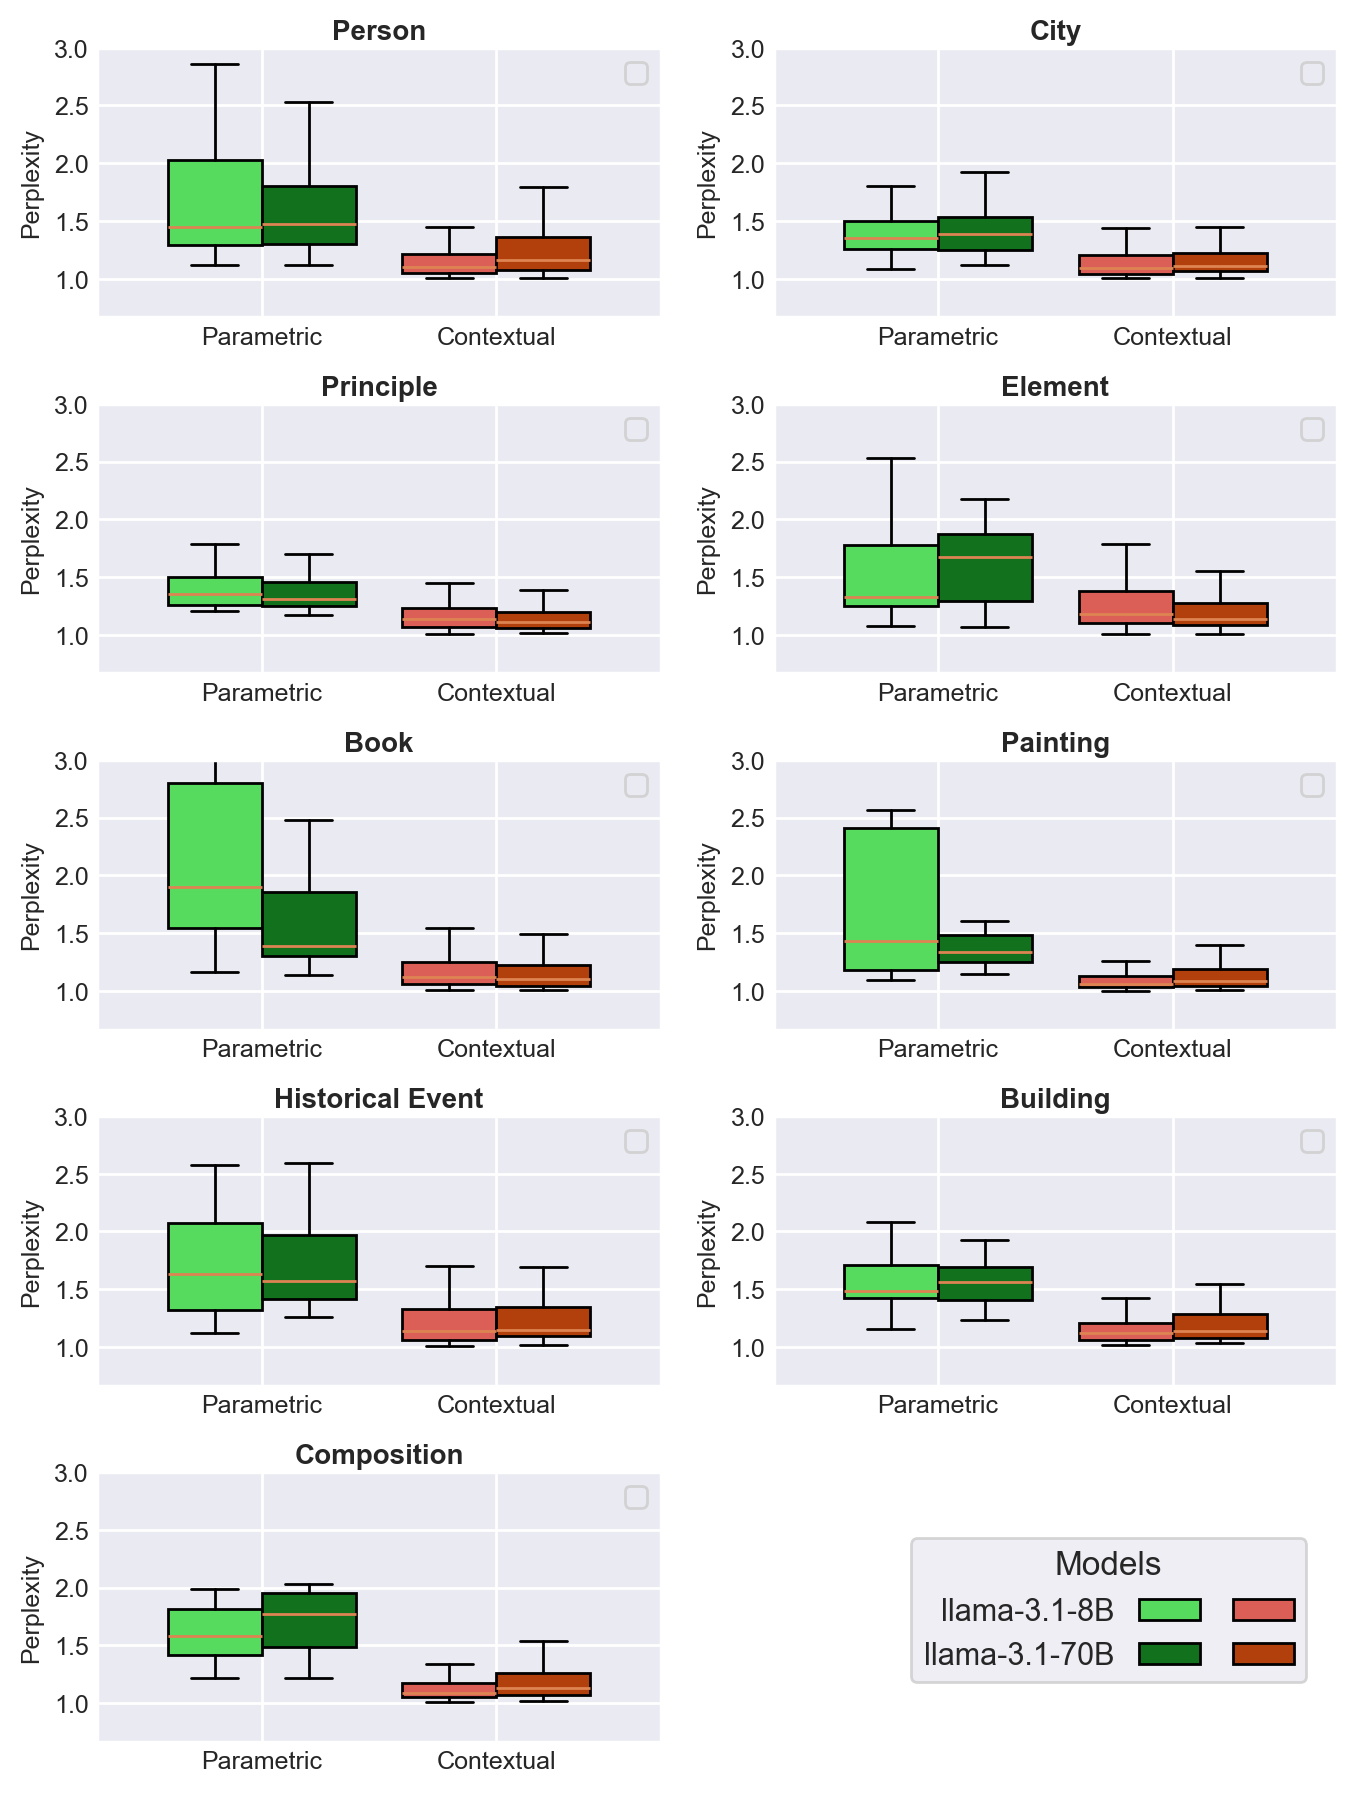
\includegraphics[width=\textwidth]{llama_catboxes.png}
	\caption{Box plots representing the distribution of the perplexities when running both Llama models, grouped by category.}
\end{figure}

\begin{figure}[p]
	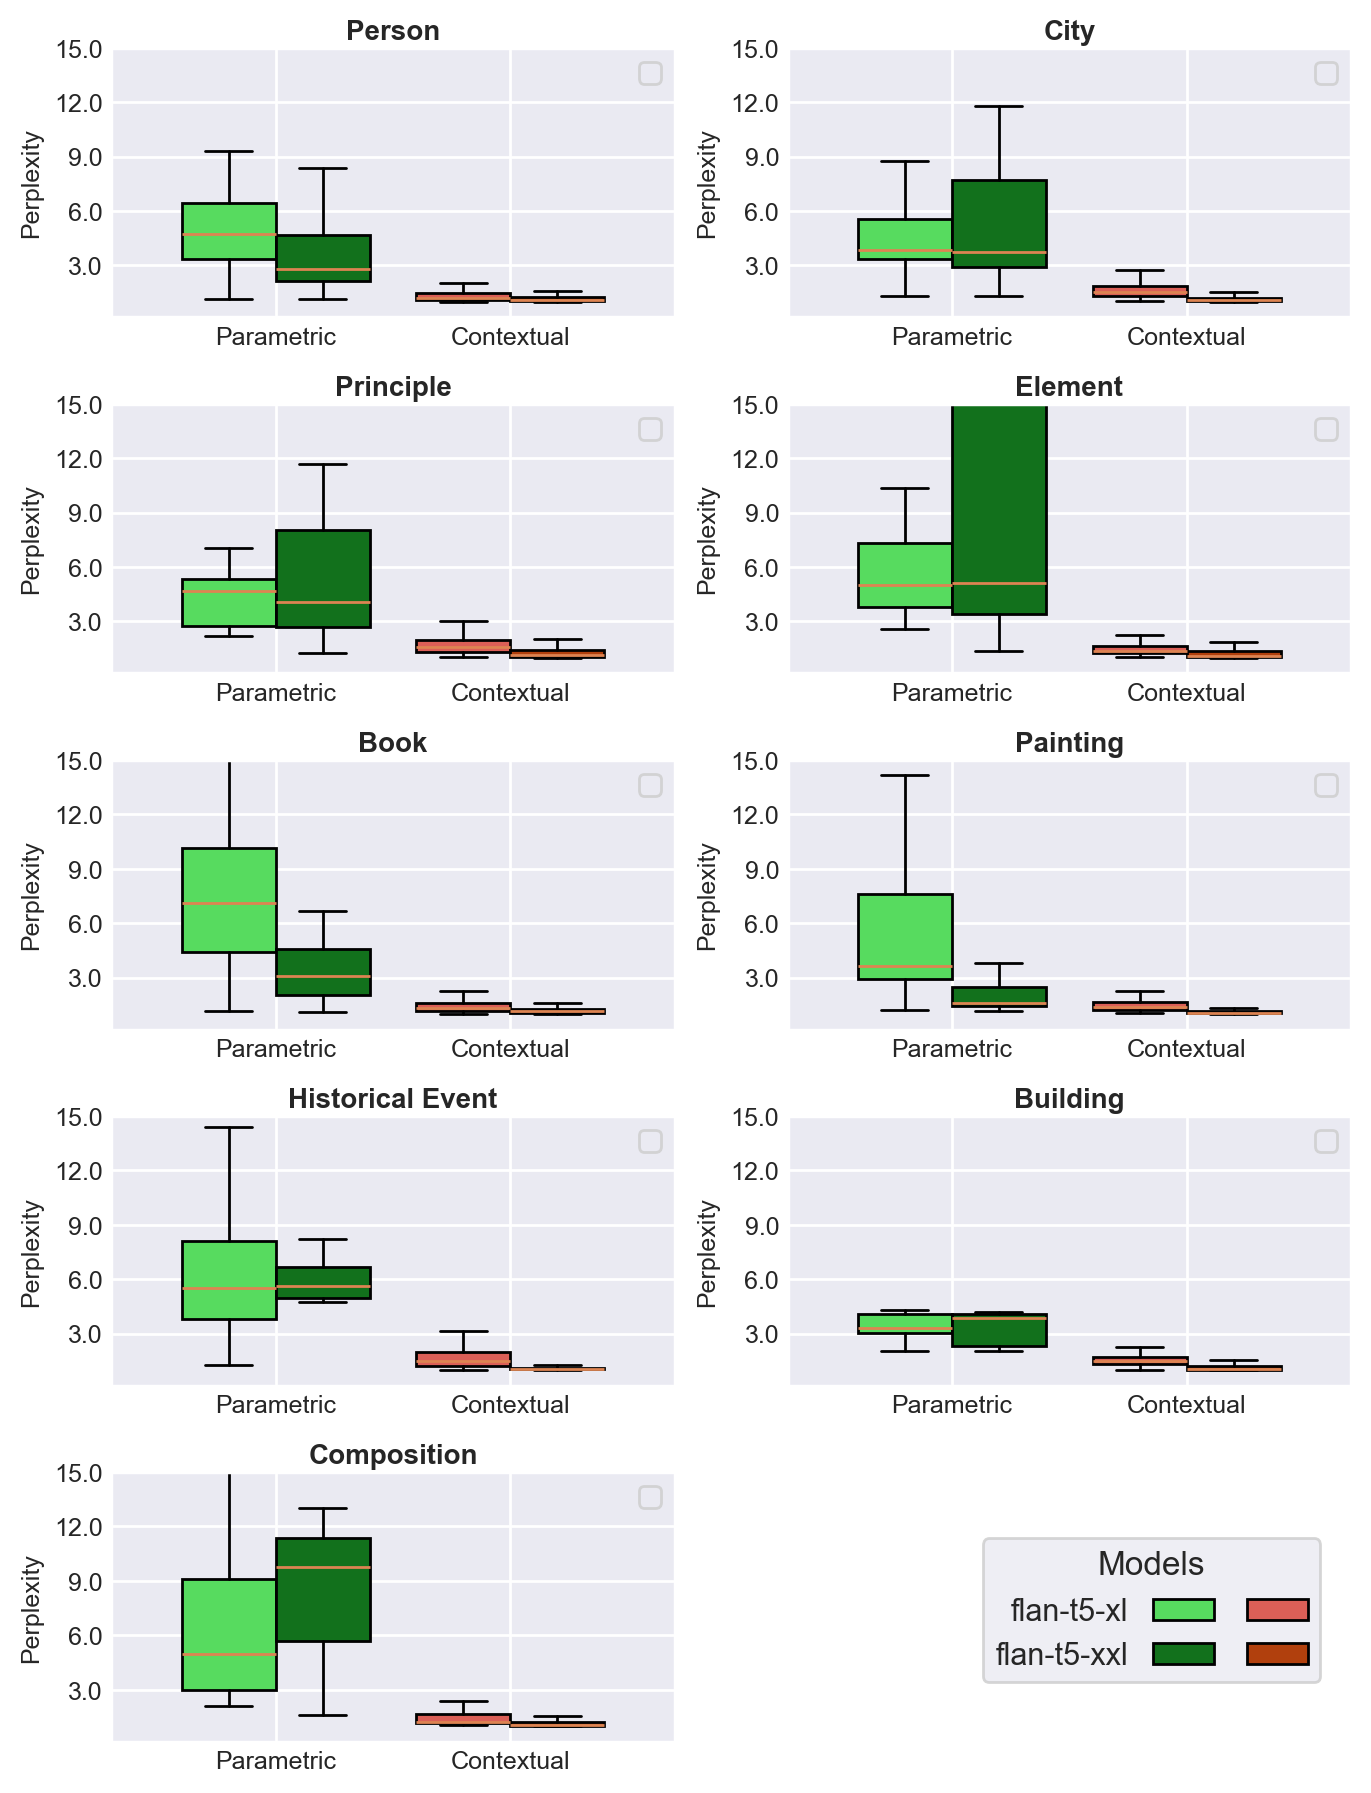
\includegraphics[width=\textwidth]{flan_catboxes.png}
	\caption{Box plots representing the distribution of the perplexities when running both Flan-T5 models, grouped by category.}
\end{figure}
